\setAuthor{Oleg Košik}
\setRound{lõppvoor}
\setYear{2006}
\setNumber{G 7}
\setDifficulty{6}
\setTopic{Termodünaamika}

\prob{Tuba}
Külmade tõttu läks küttesüsteem rikki ja temperatuur toas hakkas langema. Ühel hetkel pandi tööle ajas muutumatu võimsusega töötav soojapuhur ning temperatuur toas hakkas taas tõusma. Graafikul on toodud toatemperatuuri sõltuvus ajast. Leidke toatemperatuur pika aja möödumisel. Protsessi vältel välistingimused ei muutunud. Seinte ja toas olevate esemete soojusmahtuvusega mitte arvestada. Soojusvahetuse kiirus väliskeskkonnaga ei ole võrdeline temperatuuride vahega.

\begin{center}
	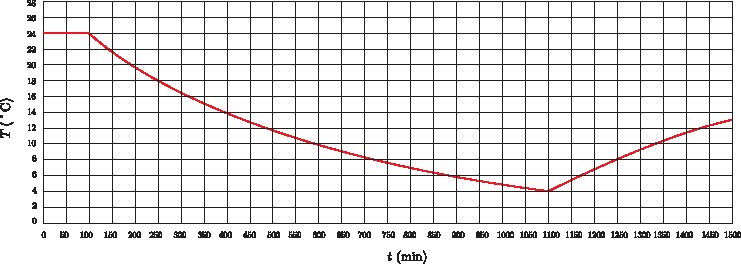
\includegraphics[width=\linewidth]{2006-v3g-07-yl}
\end{center}

\hint
Temperatuuri kasvu või langemise kiirus on võrdeline tuppa siseneva summaarse soojusliku võimsusega. Sellele vastab graafiku puutuja tõus. Tuulepuhuja sisse lülitamise ajahetkel oli graafiku tõusu muut võrdeline tuulepuhuja võimsusega.

\solu
Temperatuuri kasvu või langemise kiirus on võrdeline tuppa siseneva summaarse soojusliku võimsusega. Sellele vastab graafiku puutuja tõus. Ajahetkeni $t = \SI{1100}{min}$ läheb soojus toast välja, peale seda lisandub kaotatavale võimsusele tuulepuhuja võimsus. Tuulepuhuja võimsusele vastab puutuja tõusu muut mingil temperatuuril. Näiteks hetke $t = \SI{1100}{min}$ jaoks saame, et puutuja tõusu muut on (ligikaudu) $8/1000 + \num{10,2}/400 \approx \SI{0,036}{\degreeCelsius/min}$. Graafiku abil leiame nüüd temperatuuri, mille korral soojuskadude võimsus võrdub tuulepuhuja võimsusega. Selle jaoks võib kasutada joonlauda tõusuga \SI{0,036}{\degreeCelsius/min} ning määrata punkt graafikus, mis puutub antud sirget. Graafiku esimeses osas on selline punkt umbes temperatuuril $T = \SI{20}{\degreeCelsius}$. Seega toatemperatuur pika aja möödumisel on $T = \SI{20}{\degreeCelsius}$.
\probend